%%% fs-state-consistency - Fault tolerance

\label {fs-consistency-section}

To bridge the gap between the determinism and exactly once we need to design protocols for recovery function $F$ and saving data needed for correct restoring. In this section, we describe protocols for exactly once enforcement on top of drifting state model introduced in the previous section. While we exploit some properties of this model, proposed protocols can be generalized to any deterministic stream processing engine.

In general, determinism allows us to relax the requirement introduced in the Theorem~\ref{necessary_conditions}: output elements in a deterministic system can be delivered to end-user before results of non-commutative operations are written to persistent external storage. Hence, if data for recovery is periodically saved, the duration of this period will not affect latency.

In order to achieve exactly once on top of the drifting state model we propose the following way:
\begin{itemize}
    \item Periodically save (take a snapshot of) grouping elements to persistent storage
    \item Consistently restore groupings and replay missed input elements
    \item Ensure that output elements which have been already released will not be duplicated after recovery and input reprocessing
\end{itemize}

We do not enforce a strict architecture of the system, but assume that there are several functional agents which are demonstrated in Figure~\ref{arch}:
\begin{itemize}
    \item \Acker\ traces the items dependencies and the progress of computations. It sends monotonic in terms of $t(x)$ notifications about which elements are in the barrier.
    \item Coordinator listens notifications from~\Acker\ and manages snapshotting and recovery
    \item Cluster state manager (ZooKeeper) is used to keep service information for recovery
    \item Persistent storage is needed for reliable storing of state snapshot. In case of failures, the state snapshot is recovered from persistent storage. It can be a distributed file system or database (e.g., HDFS, S3, MongoDB, GFS, HBase, etc.).
    \item Data producer that is able to replay some set of previous input elements with the same $t(x)$. The role of $t(x)$ can be played by any monotonic sequence, e.g. offsets in Kafka
    \item Data consumer that is responsible for output elements receiving. The exact requirements for data consumer are detailed further in this section
    \item Node is an executor of user-defined operations. The computation can be balanced through the distribution of data elements among nodes. Each node has a {\em barrier} that deliver output elements to end-user. The exact barrier functionality is mentioned in section~\ref{fs-model-section}.
\end{itemize}

\subsection{Snapshotting}

\subsubsection{Grouping}

\begin{figure}[tbp]
  \centering
  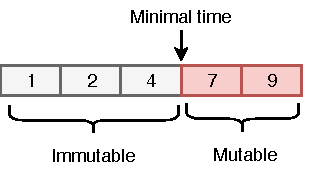
\includegraphics[width=0.5\columnwidth]{pics/immutable}
  \caption{Grouping list won't be modified up to element that corresponds to current minimal $t(x)$}    
  \label {immutable}    
\end{figure}

\begin{figure}[htbp]
  \centering
  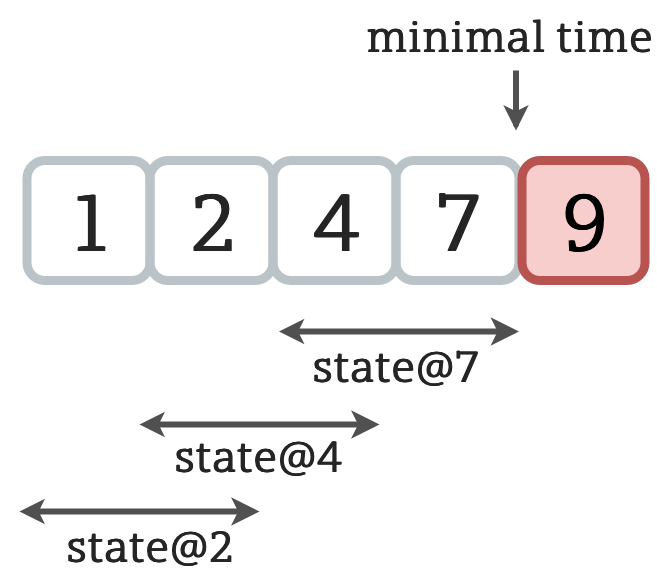
\includegraphics[width=0.5\columnwidth]{pics/substate}
  \caption{Grouping elements with window = 2. Window-sized sublists are states in terms of drifting state model}
  \label {substate}
\end{figure}

In order to periodically save grouping elements, there is a need to determine which part of them is stable and sufficient for recovery. It is convenient to use~\Acker\ notifications for this purpose. Let $t_{min}$ be the right bound of the last received notification from~\Acker. It means that all elements that have given $t(x)$ been completely processed. In other words, it is the {\em minimal} $t(x)$ of elements which are still in the system.  
Grouping's state in practice are lists sorted by $t(x)$. Because of the guarantees provided by~\Acker\ notifications, these lists will not be modified at any position before the item with $t(x)=t_{min}$. The immutable prefix and mutable suffix of grouping list are shown at Figure~\ref{immutable}. At the same time, because of the grouping semantics, state that is reached after consuming all data items with $t(x)$ in a range $[0..t_{min})$ is just a window-sized sublist that is located in the immutable part of the list, the example is shown in figure~\ref{substate}. Thereby, state snapshotting of different groupings can be done asynchronously to each other and to the computational process of the current operation. 

Considering the properties mentioned above, the protocol of grouping state snapshotting is the following:

\begin{itemize}
    \item On notification from~\Acker\, the coordinator sends a request for the new snapshot along with minimal $t(x)$
    \item When grouping operation receives the request, it asynchronously writes lists to persistent external storage and sends back the acceptance message
    \item When~\Acker\ receives all acceptance messages, it saves the $t(x)$ of the snapshot to cluster state manager
\end{itemize}

The coordinator can send requests for the new snapshot not for each minimal time event, e.g., it can skip request if the elapsed time since the last snapshot is less than some threshold. Parameters that influence the frequency of snapshots are in the user's scope. An important feature is that this parameter influences recovery time, but not the processing latency.

This protocol satisfies the following properties regarding the $t_{snap}$ that is written to cluster state manager: all groupings can restore the state that is reached after consuming all data items with $t(x)$ in a range $[0..t_{snap})$. Hence, $t_{snap}$ can be used as a resuming point after recovery without loss of consistency.

It is worth to note that the proposed protocol is similar to the state snapshotting protocol used in Flink~\cite{Carbone:2017:SMA:3137765.3137777}. The key difference is that in our method, output releasing agents (barriers) do not take part in a distributed transaction (variation of 2PC), because in a deterministic system there is no need to wait until the snapshot is taken in order to consistently release output elements. This difference determines the significant latency decrease that is demonstrated further in experiments.

\subsubsection{Last output element}

Minimal time notifications are sent by the~\Acker\ with monotonically increasing $t(x)$. Barrier receives these notifications and releases output items with monotonically increasing $t(x)$ as well. Hence, the barrier can filter out any items with $t(x)$ less than or equal to the $t(x)$ of the last released item $t_{last}$ in order to preserve exactly once after recovery. To implement this mechanism, there is a need to atomically deliver output items and update $t_{last}$. To solve this problem, we require the following output protocol with data consumer: 

\begin{itemize}
    \item When minimal time notification is received, barrier send output bundle to the data consumer. This bundle contains all corresponding output items and $t_{last}$. The consumer must acknowledge that it received the bundle
    \item Barrier does not send new output bundle until the previous one is not acknowledged
    \item Consumer must return last received bundle on barrier's request 
\end{itemize}

This protocol guarantees that $t_{last}$ and released items are always consistent with each other. It implies that the barrier can request the last released bundle and fetch $t_{last}$ after recovery to avoid duplicates which can be generated during input elements reprocessing.

Thus, on the one hand, we delegate the part of the basic functionality to data consumers. On the other hand, the requirement on data consumer is not so strong and can be naturally satisfied by real-world consumers (HDFS, Kafka, databases, etc.). 

\begin{figure*}[tbp]
  \centering
  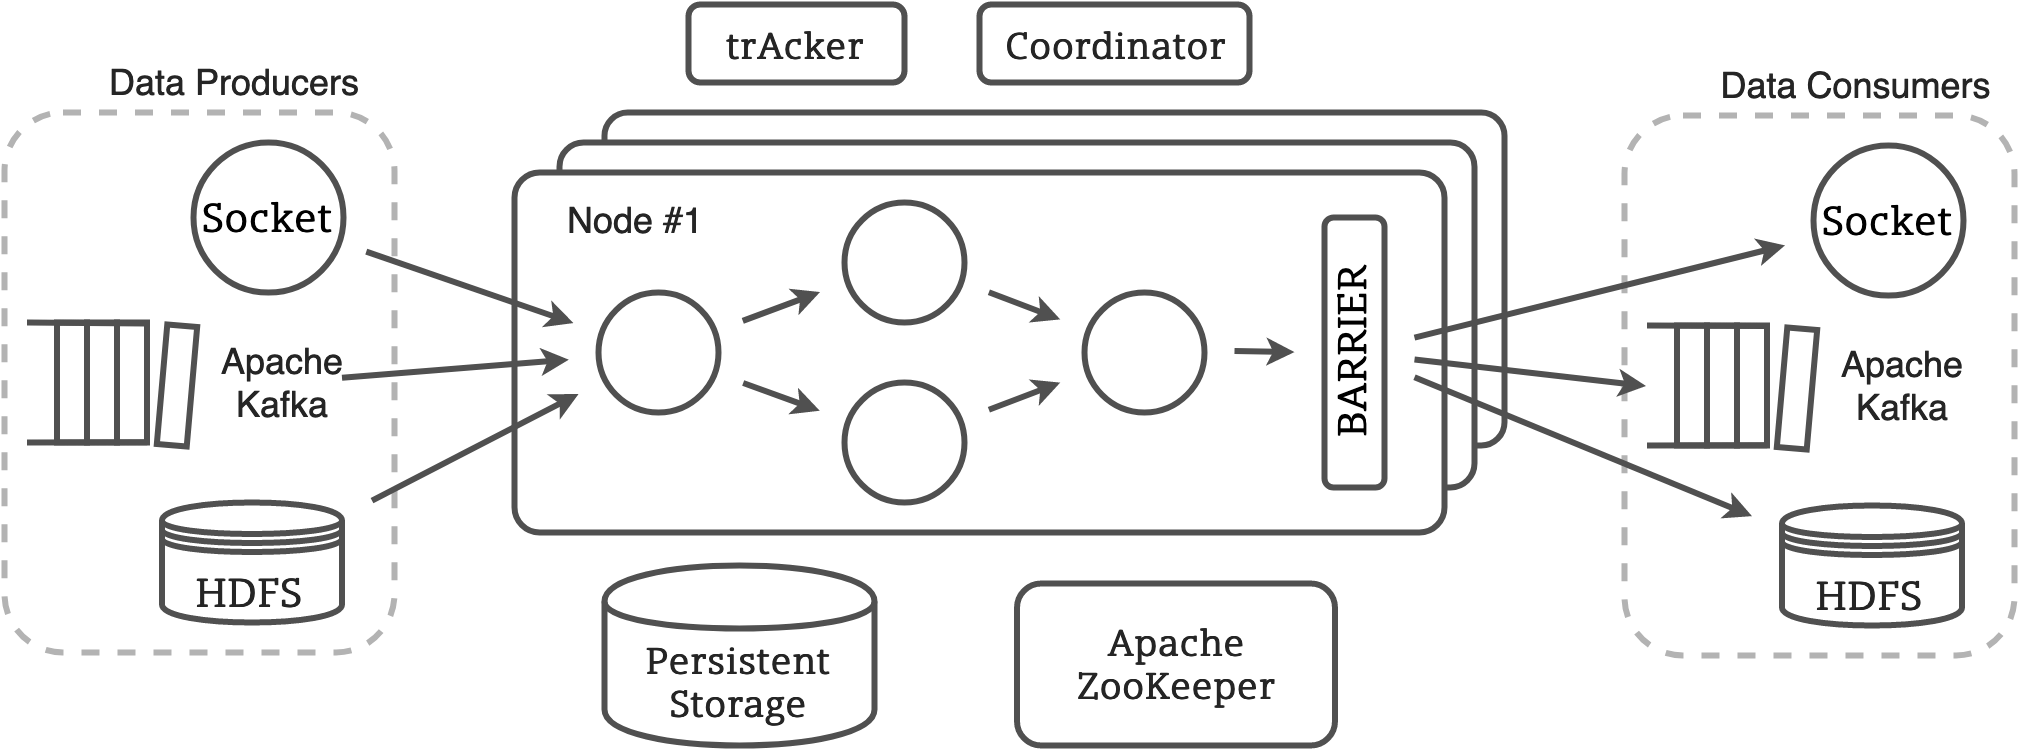
\includegraphics[width=0.78\textwidth]{pics/arch}
  \caption{The overview of an architecture for drifting state implementation}
  \label {arch}
\end{figure*}

\subsection{Failure detection and recovery}

Typically, distributed systems take into consideration the following types of failures:
\begin{itemize}
    \item Packet loss
    \item Node failure
    \item Network partitioning
\end{itemize}

Network partitioning is the special case of failure because in this case computations cannot be restarted. We believe that in this case, stream processing does not make sense. To the best of our knowledge, there are no open-source stream processing systems that tolerate network partitioning.

As it was described above,~\Acker\ traces data items using the table of XORs grouped by $t(x)$. Therefore, packet loss can be determined by the~\Acker\ because the corresponding value in~\Acker\ 's table will not be nullified. Node failure can also be observed by the~\Acker\ through periodical heartbeats. 

In case of packet loss or node failure,~\Acker\ can enforce coordinator to begin computations restart from the last successful grouping lists snapshot. The failure of the~\Acker\ itself can be detected by the cluster state manager, that triggers the same restart protocol. Restart protocol includes the following steps:

\begin{itemize}
    \item Coordinator reads $t(x)$ of the last snapshot from a cluster state manager. After that, it broadcasts this $t(x)$ to all grouping operations
    \item Grouping operations fetch their states from state storage. After that, grouping operations send an acknowledgment that they are ready for processing to the coordinator 
    \item Barriers request the last released bundle from data consumers and send acknowledgments that they are ready for processing to the coordinator
    \item When the coordinator receives all acknowledgments from groupings and barriers, it requests data producer to replay starting from the $t(x)$ of the last snapshot  
\end{itemize}

Proposed protocol guarantees the following properties that allow preserving exactly once:

\begin{itemize}
    \item Processing does not restart until all grouping operations obtain consistent states. The consistency of these states is guaranteed by the state snapshotting protocol. Therefore, the elements are not lost.
    \item Duplicates are not produced because, at the moment when processing is restarted, it is ensured that barrier has obtained the last released $t(x)$ and is able to filter out extra items.
\end{itemize}